\section{Positionsbestimmung}
\begin{frame}
    \frametitle{\insertsection}

    

\end{frame}


\section{Potentiometrische Wegaufnehmer}
\begin{frame}
    \frametitle{\insertsection}

    

\end{frame}


\section{Induktive Wegaufnehmer}
\begin{frame}
    \frametitle{\insertsection}

    \begin{columns}[onlytextwidth]
        \begin{column}[t]{0.5\textwidth}
            \begin{itemize}
                \item Sehr robust bei widrigen Umweltbedingungen (z.B. Wasser, Schmutz,…)
                \item Indirekte Messung des Abstands über Luftspalt- oder Flussänderung
                \begin{itemize}
                    \item Induktivitätsänderung $dL$ über Stromänderungsmessung
                    \item Berührungslose Messung 
                \end{itemize}
                \item Offene und geschlossene Bauform
                \begin{itemize}
                    \item Geschlossen: Drosselkern wird über Joch am Messobjekt geschlossen
                    \item Offen: Feldverteilung des offenen Kerns wird durch Objekt verändert (materialabhängig)
                \end{itemize}
                \item Nahbereichssensor mit extrem hoher Ortsauflösung
            \end{itemize}
        \end{column}
        \begin{column}[t]{0.48\textwidth}
            \begin{figure}
                \vspace{-1cm}
                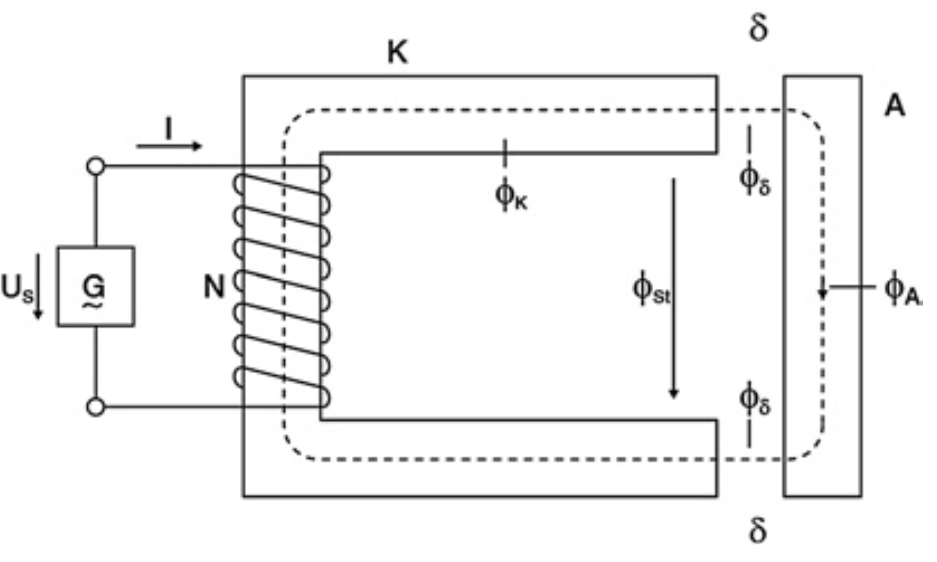
\includegraphics[width=0.8\textwidth]{fig/traenkler_2012_abb_10_3}
                \caption{Magnetischer Kreis mit Drosselspule und Queranker, aus \cite{traenkler2014}.}
            \end{figure}
            \begin{gather*}
                u = L \frac{d i}{d t} = -n \frac{d \Phi}{d t}\\
                \Rightarrow L = N \frac{d \Phi}{d i} = \frac{N^2}{R_{\textrm{m}}}
            \end{gather*}
            Mit mag. Widerstand $R_{\textrm{m}} = \frac{\oint \vec{H} d \vec{l}}{\Phi}$
        \end{column}
    \end{columns}

\end{frame}